\section{Working with \rt transit data}
\label{sec:gtfs}

GTFS (general transit feed specification)
is an API (application programming interface) specification for transit data
detailing how it should be organised,
making access easier for application developers.
Developed and maintained by Google \citep{GoogleDevelopers_2006},
who use it in Google Maps Transit Directions,
it is used by over 900~transit providers around the world,
including here in Auckland, New Zealand
(source \url{http://transitfeeds.com}).
An advantage of this standardised format is that,
provided an application depends solely on GTFS data,
after developing it locally in Auckland it can be deployed to any other GTFS-based
public transport system with minimal modification.


There are two components to GTFS.
The first, \emph{GTFS static}, includes information about
\begin{itemize}
\item \emph{stops}, a physical location where passengers can embark and disembark the vehicle;
\item \emph{routes}, a sequence of two or more stops displayed as a single service;
\item \emph{trips}, an instance of a route occuring at a specific time of day;
\item \emph{schedules}, specifying the arrival (and departure) times for each bus at each of its stops; 
\item \emph{shapes}, the sequence of points defining a vehicle's path along a route
\end{itemize}
\citep{GoogleDevelopers_2006}.
The second component is \emph{GTFS realtime},
which is only available in a subset of the providers due to the requirement of 
onboard GPS tracking devices and a central server.
It provides a standardised format for sharing vehicle positions and trip delays,
and are typically accessed by developers via an API can be used in \rt applications.

As mentioned in Section~\ref{sec:intro},
there are some major issues with the current prediction method in Auckland.
These are almost directly attributed to GTFS-realtime trip updates,
which are currently the sole source of data for ETAs.
Trip updates are reported whenever a vehicle arrives or departs a stop,
and includes the delay between the scheduled and actual arrival times,
and is propagated to all future stops to adjust their ETAs.
This assumes that the schedule is well calibrated and the time between scheduled arrivals
is representative of the real-world travel time between stops. 
Therefore, an alternative estimation approach using \rt travel times 
between stops is more adequate.



\subsection{Transit network construction}
\label{sec:network_build}

The primary predictor of arrival time is 
the travel time along roads between where the bus is \emph{now},
and the stop at which the passenger is waiting.
In most applications, however, this vital information is unavailable,
at least directly,
so here we construct a transit road network consisting of intersections
and the roads between them.
By generalising to physical roads,
we remove any route-dependency,
which increases the quantity of data available for each road.
Each route is then represeted as a sequence of road segments,
each with an associated travel time.


The transit network is constructed by splitting each route
into spatially identifiable segments,
each representative of a physical road.
The simplest way to do this is to use bus stops as nodes in the network
(Figure~\ref{fig:network_creation_1}),
and connecting roads as edges.
In this way, routes that serice the same subsequence of stops
will all contribute to congestion information for the connecting roads,
as shown in Figure~\ref{fig:network_creation_2}.
There are several drawbacks to this method,
for example routes merge at physical intersections, not bus stops,
so some overlap will occur as shown.
However, this is minimal, and our simplification is sufficent for the current work.


\begin{figure}[tb]
    \centering
    \begin{subfigure}{0.7\textwidth}
        \centering
        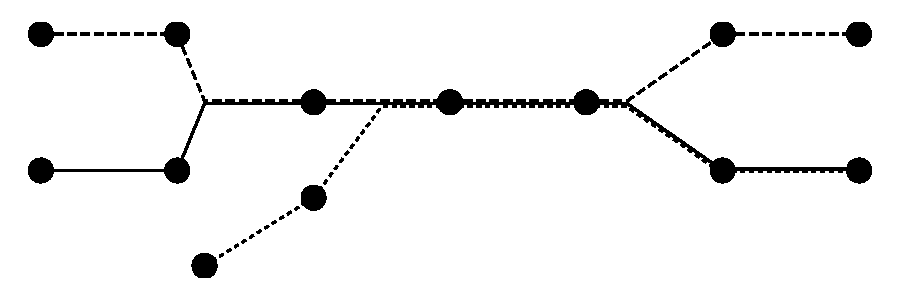
\includegraphics[width=0.95\textwidth]{figures/02_network_segments_1.pdf}
        \caption{Raw GTFS route shapes}
        \label{fig:network_creation_1}
    \end{subfigure} \\
    \begin{subfigure}{0.7\textwidth}
        \centering
        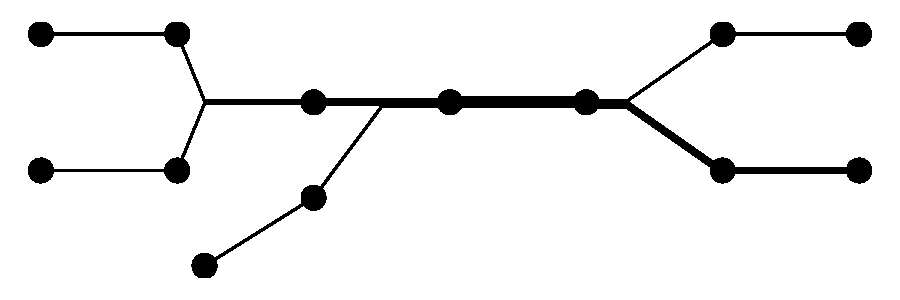
\includegraphics[width=0.95\textwidth]{figures/02_network_segments_2.pdf}
        \caption{GTFS-based road network}
        \label{fig:network_creation_2}
    \end{subfigure}
    \caption{Construction of a route network involves combining routes at nodes %
        (here we are using stops) which are connected by edges (roads). %
        In (a), the three unique routes, represented by different line types, clearly %
        overlap in several places. In (b) these have been merged, and the width of each line %
        represents how many routes use that link.}
    \label{fig:network_creation}
\end{figure}


\subsection{Realtime vehicle locations}
\label{sec:realtime_data}

GTFS-realtime provides the current positions of vehicles in a transit network.
The data consists of the time $t_k$ that the observation was made,
the GPS position of the vehicle, $\bY_k$, 
and information about the trip being serviced.
In Auckland, vehicle positions are updated with a frequency of anywhere between 10~seconds and several minutes,
so there is often a lot of uncertainty about a vehicle's intermediate trajectory,
particularly when there are one or more bus stops along the way.
It is also possible for a bus to remain stationary,
for example due to heavy congestion,
so the number of possible trajectories rapidly increases with 
the time between observations.


One important consideration regarding Auckland Transport's \rt implementation is that
buses are programmed to report their location when arriving at or departing from
bus stops, as well as some major intersections.
To further complicate this,
these positions can be pre-emtive,
(i.e., the bus is almost there, but not quite),
so consecutive observations can show a bus traveling backwards.
To handle this, we compute the approximate distance traveled, $\tilde x_k$,
of the vehicle by finding the nearest point on the path to the observation;
if this has decreased, the current state is rejected and the vehicle reverted
to its previous state before continuing.
This way, we avoid degeneration of the particle fitler (Section~\ref{sec:model_perf})
at the cost of losing one observation that is most likely invalid anyway.

